
\documentclass{article} % For LaTeX2e
\usepackage{iclr2020_conference,times}

% Optional math commands from https://github.com/goodfeli/dlbook_notation.
%%%%% NEW MATH DEFINITIONS %%%%%

\usepackage{amsmath,amsfonts,bm}

% Mark sections of captions for referring to divisions of figures
\newcommand{\figleft}{{\em (Left)}}
\newcommand{\figcenter}{{\em (Center)}}
\newcommand{\figright}{{\em (Right)}}
\newcommand{\figtop}{{\em (Top)}}
\newcommand{\figbottom}{{\em (Bottom)}}
\newcommand{\captiona}{{\em (a)}}
\newcommand{\captionb}{{\em (b)}}
\newcommand{\captionc}{{\em (c)}}
\newcommand{\captiond}{{\em (d)}}

% Highlight a newly defined term
\newcommand{\newterm}[1]{{\bf #1}}


% Figure reference, lower-case.
\def\figref#1{figure~\ref{#1}}
% Figure reference, capital. For start of sentence
\def\Figref#1{Figure~\ref{#1}}
\def\twofigref#1#2{figures \ref{#1} and \ref{#2}}
\def\quadfigref#1#2#3#4{figures \ref{#1}, \ref{#2}, \ref{#3} and \ref{#4}}
% Section reference, lower-case.
\def\secref#1{section~\ref{#1}}
% Section reference, capital.
\def\Secref#1{Section~\ref{#1}}
% Reference to two sections.
\def\twosecrefs#1#2{sections \ref{#1} and \ref{#2}}
% Reference to three sections.
\def\secrefs#1#2#3{sections \ref{#1}, \ref{#2} and \ref{#3}}
% Reference to an equation, lower-case.
\def\eqref#1{equation~\ref{#1}}
% Reference to an equation, upper case
\def\Eqref#1{Equation~\ref{#1}}
% A raw reference to an equation---avoid using if possible
\def\plaineqref#1{\ref{#1}}
% Reference to a chapter, lower-case.
\def\chapref#1{chapter~\ref{#1}}
% Reference to an equation, upper case.
\def\Chapref#1{Chapter~\ref{#1}}
% Reference to a range of chapters
\def\rangechapref#1#2{chapters\ref{#1}--\ref{#2}}
% Reference to an algorithm, lower-case.
\def\algref#1{algorithm~\ref{#1}}
% Reference to an algorithm, upper case.
\def\Algref#1{Algorithm~\ref{#1}}
\def\twoalgref#1#2{algorithms \ref{#1} and \ref{#2}}
\def\Twoalgref#1#2{Algorithms \ref{#1} and \ref{#2}}
% Reference to a part, lower case
\def\partref#1{part~\ref{#1}}
% Reference to a part, upper case
\def\Partref#1{Part~\ref{#1}}
\def\twopartref#1#2{parts \ref{#1} and \ref{#2}}

\def\ceil#1{\lceil #1 \rceil}
\def\floor#1{\lfloor #1 \rfloor}
\def\1{\bm{1}}
\newcommand{\train}{\mathcal{D}}
\newcommand{\valid}{\mathcal{D_{\mathrm{valid}}}}
\newcommand{\test}{\mathcal{D_{\mathrm{test}}}}

\def\eps{{\epsilon}}


% Random variables
\def\reta{{\textnormal{$\eta$}}}
\def\ra{{\textnormal{a}}}
\def\rb{{\textnormal{b}}}
\def\rc{{\textnormal{c}}}
\def\rd{{\textnormal{d}}}
\def\re{{\textnormal{e}}}
\def\rf{{\textnormal{f}}}
\def\rg{{\textnormal{g}}}
\def\rh{{\textnormal{h}}}
\def\ri{{\textnormal{i}}}
\def\rj{{\textnormal{j}}}
\def\rk{{\textnormal{k}}}
\def\rl{{\textnormal{l}}}
% rm is already a command, just don't name any random variables m
\def\rn{{\textnormal{n}}}
\def\ro{{\textnormal{o}}}
\def\rp{{\textnormal{p}}}
\def\rq{{\textnormal{q}}}
\def\rr{{\textnormal{r}}}
\def\rs{{\textnormal{s}}}
\def\rt{{\textnormal{t}}}
\def\ru{{\textnormal{u}}}
\def\rv{{\textnormal{v}}}
\def\rw{{\textnormal{w}}}
\def\rx{{\textnormal{x}}}
\def\ry{{\textnormal{y}}}
\def\rz{{\textnormal{z}}}

% Random vectors
\def\rvepsilon{{\mathbf{\epsilon}}}
\def\rvtheta{{\mathbf{\theta}}}
\def\rva{{\mathbf{a}}}
\def\rvb{{\mathbf{b}}}
\def\rvc{{\mathbf{c}}}
\def\rvd{{\mathbf{d}}}
\def\rve{{\mathbf{e}}}
\def\rvf{{\mathbf{f}}}
\def\rvg{{\mathbf{g}}}
\def\rvh{{\mathbf{h}}}
\def\rvu{{\mathbf{i}}}
\def\rvj{{\mathbf{j}}}
\def\rvk{{\mathbf{k}}}
\def\rvl{{\mathbf{l}}}
\def\rvm{{\mathbf{m}}}
\def\rvn{{\mathbf{n}}}
\def\rvo{{\mathbf{o}}}
\def\rvp{{\mathbf{p}}}
\def\rvq{{\mathbf{q}}}
\def\rvr{{\mathbf{r}}}
\def\rvs{{\mathbf{s}}}
\def\rvt{{\mathbf{t}}}
\def\rvu{{\mathbf{u}}}
\def\rvv{{\mathbf{v}}}
\def\rvw{{\mathbf{w}}}
\def\rvx{{\mathbf{x}}}
\def\rvy{{\mathbf{y}}}
\def\rvz{{\mathbf{z}}}

% Elements of random vectors
\def\erva{{\textnormal{a}}}
\def\ervb{{\textnormal{b}}}
\def\ervc{{\textnormal{c}}}
\def\ervd{{\textnormal{d}}}
\def\erve{{\textnormal{e}}}
\def\ervf{{\textnormal{f}}}
\def\ervg{{\textnormal{g}}}
\def\ervh{{\textnormal{h}}}
\def\ervi{{\textnormal{i}}}
\def\ervj{{\textnormal{j}}}
\def\ervk{{\textnormal{k}}}
\def\ervl{{\textnormal{l}}}
\def\ervm{{\textnormal{m}}}
\def\ervn{{\textnormal{n}}}
\def\ervo{{\textnormal{o}}}
\def\ervp{{\textnormal{p}}}
\def\ervq{{\textnormal{q}}}
\def\ervr{{\textnormal{r}}}
\def\ervs{{\textnormal{s}}}
\def\ervt{{\textnormal{t}}}
\def\ervu{{\textnormal{u}}}
\def\ervv{{\textnormal{v}}}
\def\ervw{{\textnormal{w}}}
\def\ervx{{\textnormal{x}}}
\def\ervy{{\textnormal{y}}}
\def\ervz{{\textnormal{z}}}

% Random matrices
\def\rmA{{\mathbf{A}}}
\def\rmB{{\mathbf{B}}}
\def\rmC{{\mathbf{C}}}
\def\rmD{{\mathbf{D}}}
\def\rmE{{\mathbf{E}}}
\def\rmF{{\mathbf{F}}}
\def\rmG{{\mathbf{G}}}
\def\rmH{{\mathbf{H}}}
\def\rmI{{\mathbf{I}}}
\def\rmJ{{\mathbf{J}}}
\def\rmK{{\mathbf{K}}}
\def\rmL{{\mathbf{L}}}
\def\rmM{{\mathbf{M}}}
\def\rmN{{\mathbf{N}}}
\def\rmO{{\mathbf{O}}}
\def\rmP{{\mathbf{P}}}
\def\rmQ{{\mathbf{Q}}}
\def\rmR{{\mathbf{R}}}
\def\rmS{{\mathbf{S}}}
\def\rmT{{\mathbf{T}}}
\def\rmU{{\mathbf{U}}}
\def\rmV{{\mathbf{V}}}
\def\rmW{{\mathbf{W}}}
\def\rmX{{\mathbf{X}}}
\def\rmY{{\mathbf{Y}}}
\def\rmZ{{\mathbf{Z}}}

% Elements of random matrices
\def\ermA{{\textnormal{A}}}
\def\ermB{{\textnormal{B}}}
\def\ermC{{\textnormal{C}}}
\def\ermD{{\textnormal{D}}}
\def\ermE{{\textnormal{E}}}
\def\ermF{{\textnormal{F}}}
\def\ermG{{\textnormal{G}}}
\def\ermH{{\textnormal{H}}}
\def\ermI{{\textnormal{I}}}
\def\ermJ{{\textnormal{J}}}
\def\ermK{{\textnormal{K}}}
\def\ermL{{\textnormal{L}}}
\def\ermM{{\textnormal{M}}}
\def\ermN{{\textnormal{N}}}
\def\ermO{{\textnormal{O}}}
\def\ermP{{\textnormal{P}}}
\def\ermQ{{\textnormal{Q}}}
\def\ermR{{\textnormal{R}}}
\def\ermS{{\textnormal{S}}}
\def\ermT{{\textnormal{T}}}
\def\ermU{{\textnormal{U}}}
\def\ermV{{\textnormal{V}}}
\def\ermW{{\textnormal{W}}}
\def\ermX{{\textnormal{X}}}
\def\ermY{{\textnormal{Y}}}
\def\ermZ{{\textnormal{Z}}}

% Vectors
\def\vzero{{\bm{0}}}
\def\vone{{\bm{1}}}
\def\vmu{{\bm{\mu}}}
\def\vtheta{{\bm{\theta}}}
\def\va{{\bm{a}}}
\def\vb{{\bm{b}}}
\def\vc{{\bm{c}}}
\def\vd{{\bm{d}}}
\def\ve{{\bm{e}}}
\def\vf{{\bm{f}}}
\def\vg{{\bm{g}}}
\def\vh{{\bm{h}}}
\def\vi{{\bm{i}}}
\def\vj{{\bm{j}}}
\def\vk{{\bm{k}}}
\def\vl{{\bm{l}}}
\def\vm{{\bm{m}}}
\def\vn{{\bm{n}}}
\def\vo{{\bm{o}}}
\def\vp{{\bm{p}}}
\def\vq{{\bm{q}}}
\def\vr{{\bm{r}}}
\def\vs{{\bm{s}}}
\def\vt{{\bm{t}}}
\def\vu{{\bm{u}}}
\def\vv{{\bm{v}}}
\def\vw{{\bm{w}}}
\def\vx{{\bm{x}}}
\def\vy{{\bm{y}}}
\def\vz{{\bm{z}}}

% Elements of vectors
\def\evalpha{{\alpha}}
\def\evbeta{{\beta}}
\def\evepsilon{{\epsilon}}
\def\evlambda{{\lambda}}
\def\evomega{{\omega}}
\def\evmu{{\mu}}
\def\evpsi{{\psi}}
\def\evsigma{{\sigma}}
\def\evtheta{{\theta}}
\def\eva{{a}}
\def\evb{{b}}
\def\evc{{c}}
\def\evd{{d}}
\def\eve{{e}}
\def\evf{{f}}
\def\evg{{g}}
\def\evh{{h}}
\def\evi{{i}}
\def\evj{{j}}
\def\evk{{k}}
\def\evl{{l}}
\def\evm{{m}}
\def\evn{{n}}
\def\evo{{o}}
\def\evp{{p}}
\def\evq{{q}}
\def\evr{{r}}
\def\evs{{s}}
\def\evt{{t}}
\def\evu{{u}}
\def\evv{{v}}
\def\evw{{w}}
\def\evx{{x}}
\def\evy{{y}}
\def\evz{{z}}

% Matrix
\def\mA{{\bm{A}}}
\def\mB{{\bm{B}}}
\def\mC{{\bm{C}}}
\def\mD{{\bm{D}}}
\def\mE{{\bm{E}}}
\def\mF{{\bm{F}}}
\def\mG{{\bm{G}}}
\def\mH{{\bm{H}}}
\def\mI{{\bm{I}}}
\def\mJ{{\bm{J}}}
\def\mK{{\bm{K}}}
\def\mL{{\bm{L}}}
\def\mM{{\bm{M}}}
\def\mN{{\bm{N}}}
\def\mO{{\bm{O}}}
\def\mP{{\bm{P}}}
\def\mQ{{\bm{Q}}}
\def\mR{{\bm{R}}}
\def\mS{{\bm{S}}}
\def\mT{{\bm{T}}}
\def\mU{{\bm{U}}}
\def\mV{{\bm{V}}}
\def\mW{{\bm{W}}}
\def\mX{{\bm{X}}}
\def\mY{{\bm{Y}}}
\def\mZ{{\bm{Z}}}
\def\mBeta{{\bm{\beta}}}
\def\mPhi{{\bm{\Phi}}}
\def\mLambda{{\bm{\Lambda}}}
\def\mSigma{{\bm{\Sigma}}}

% Tensor
\DeclareMathAlphabet{\mathsfit}{\encodingdefault}{\sfdefault}{m}{sl}
\SetMathAlphabet{\mathsfit}{bold}{\encodingdefault}{\sfdefault}{bx}{n}
\newcommand{\tens}[1]{\bm{\mathsfit{#1}}}
\def\tA{{\tens{A}}}
\def\tB{{\tens{B}}}
\def\tC{{\tens{C}}}
\def\tD{{\tens{D}}}
\def\tE{{\tens{E}}}
\def\tF{{\tens{F}}}
\def\tG{{\tens{G}}}
\def\tH{{\tens{H}}}
\def\tI{{\tens{I}}}
\def\tJ{{\tens{J}}}
\def\tK{{\tens{K}}}
\def\tL{{\tens{L}}}
\def\tM{{\tens{M}}}
\def\tN{{\tens{N}}}
\def\tO{{\tens{O}}}
\def\tP{{\tens{P}}}
\def\tQ{{\tens{Q}}}
\def\tR{{\tens{R}}}
\def\tS{{\tens{S}}}
\def\tT{{\tens{T}}}
\def\tU{{\tens{U}}}
\def\tV{{\tens{V}}}
\def\tW{{\tens{W}}}
\def\tX{{\tens{X}}}
\def\tY{{\tens{Y}}}
\def\tZ{{\tens{Z}}}


% Graph
\def\gA{{\mathcal{A}}}
\def\gB{{\mathcal{B}}}
\def\gC{{\mathcal{C}}}
\def\gD{{\mathcal{D}}}
\def\gE{{\mathcal{E}}}
\def\gF{{\mathcal{F}}}
\def\gG{{\mathcal{G}}}
\def\gH{{\mathcal{H}}}
\def\gI{{\mathcal{I}}}
\def\gJ{{\mathcal{J}}}
\def\gK{{\mathcal{K}}}
\def\gL{{\mathcal{L}}}
\def\gM{{\mathcal{M}}}
\def\gN{{\mathcal{N}}}
\def\gO{{\mathcal{O}}}
\def\gP{{\mathcal{P}}}
\def\gQ{{\mathcal{Q}}}
\def\gR{{\mathcal{R}}}
\def\gS{{\mathcal{S}}}
\def\gT{{\mathcal{T}}}
\def\gU{{\mathcal{U}}}
\def\gV{{\mathcal{V}}}
\def\gW{{\mathcal{W}}}
\def\gX{{\mathcal{X}}}
\def\gY{{\mathcal{Y}}}
\def\gZ{{\mathcal{Z}}}

% Sets
\def\sA{{\mathbb{A}}}
\def\sB{{\mathbb{B}}}
\def\sC{{\mathbb{C}}}
\def\sD{{\mathbb{D}}}
% Don't use a set called E, because this would be the same as our symbol
% for expectation.
\def\sF{{\mathbb{F}}}
\def\sG{{\mathbb{G}}}
\def\sH{{\mathbb{H}}}
\def\sI{{\mathbb{I}}}
\def\sJ{{\mathbb{J}}}
\def\sK{{\mathbb{K}}}
\def\sL{{\mathbb{L}}}
\def\sM{{\mathbb{M}}}
\def\sN{{\mathbb{N}}}
\def\sO{{\mathbb{O}}}
\def\sP{{\mathbb{P}}}
\def\sQ{{\mathbb{Q}}}
\def\sR{{\mathbb{R}}}
\def\sS{{\mathbb{S}}}
\def\sT{{\mathbb{T}}}
\def\sU{{\mathbb{U}}}
\def\sV{{\mathbb{V}}}
\def\sW{{\mathbb{W}}}
\def\sX{{\mathbb{X}}}
\def\sY{{\mathbb{Y}}}
\def\sZ{{\mathbb{Z}}}

% Entries of a matrix
\def\emLambda{{\Lambda}}
\def\emA{{A}}
\def\emB{{B}}
\def\emC{{C}}
\def\emD{{D}}
\def\emE{{E}}
\def\emF{{F}}
\def\emG{{G}}
\def\emH{{H}}
\def\emI{{I}}
\def\emJ{{J}}
\def\emK{{K}}
\def\emL{{L}}
\def\emM{{M}}
\def\emN{{N}}
\def\emO{{O}}
\def\emP{{P}}
\def\emQ{{Q}}
\def\emR{{R}}
\def\emS{{S}}
\def\emT{{T}}
\def\emU{{U}}
\def\emV{{V}}
\def\emW{{W}}
\def\emX{{X}}
\def\emY{{Y}}
\def\emZ{{Z}}
\def\emSigma{{\Sigma}}

% entries of a tensor
% Same font as tensor, without \bm wrapper
\newcommand{\etens}[1]{\mathsfit{#1}}
\def\etLambda{{\etens{\Lambda}}}
\def\etA{{\etens{A}}}
\def\etB{{\etens{B}}}
\def\etC{{\etens{C}}}
\def\etD{{\etens{D}}}
\def\etE{{\etens{E}}}
\def\etF{{\etens{F}}}
\def\etG{{\etens{G}}}
\def\etH{{\etens{H}}}
\def\etI{{\etens{I}}}
\def\etJ{{\etens{J}}}
\def\etK{{\etens{K}}}
\def\etL{{\etens{L}}}
\def\etM{{\etens{M}}}
\def\etN{{\etens{N}}}
\def\etO{{\etens{O}}}
\def\etP{{\etens{P}}}
\def\etQ{{\etens{Q}}}
\def\etR{{\etens{R}}}
\def\etS{{\etens{S}}}
\def\etT{{\etens{T}}}
\def\etU{{\etens{U}}}
\def\etV{{\etens{V}}}
\def\etW{{\etens{W}}}
\def\etX{{\etens{X}}}
\def\etY{{\etens{Y}}}
\def\etZ{{\etens{Z}}}

% The true underlying data generating distribution
\newcommand{\pdata}{p_{\rm{data}}}
% The empirical distribution defined by the training set
\newcommand{\ptrain}{\hat{p}_{\rm{data}}}
\newcommand{\Ptrain}{\hat{P}_{\rm{data}}}
% The model distribution
\newcommand{\pmodel}{p_{\rm{model}}}
\newcommand{\Pmodel}{P_{\rm{model}}}
\newcommand{\ptildemodel}{\tilde{p}_{\rm{model}}}
% Stochastic autoencoder distributions
\newcommand{\pencode}{p_{\rm{encoder}}}
\newcommand{\pdecode}{p_{\rm{decoder}}}
\newcommand{\precons}{p_{\rm{reconstruct}}}

\newcommand{\laplace}{\mathrm{Laplace}} % Laplace distribution

\newcommand{\E}{\mathbb{E}}
\newcommand{\Ls}{\mathcal{L}}
\newcommand{\R}{\mathbb{R}}
\newcommand{\emp}{\tilde{p}}
\newcommand{\lr}{\alpha}
\newcommand{\reg}{\lambda}
\newcommand{\rect}{\mathrm{rectifier}}
\newcommand{\softmax}{\mathrm{softmax}}
\newcommand{\sigmoid}{\sigma}
\newcommand{\softplus}{\zeta}
\newcommand{\KL}{D_{\mathrm{KL}}}
\newcommand{\Var}{\mathrm{Var}}
\newcommand{\standarderror}{\mathrm{SE}}
\newcommand{\Cov}{\mathrm{Cov}}
% Wolfram Mathworld says $L^2$ is for function spaces and $\ell^2$ is for vectors
% But then they seem to use $L^2$ for vectors throughout the site, and so does
% wikipedia.
\newcommand{\normlzero}{L^0}
\newcommand{\normlone}{L^1}
\newcommand{\normltwo}{L^2}
\newcommand{\normlp}{L^p}
\newcommand{\normmax}{L^\infty}

\newcommand{\parents}{Pa} % See usage in notation.tex. Chosen to match Daphne's book.

\DeclareMathOperator*{\argmax}{arg\,max}
\DeclareMathOperator*{\argmin}{arg\,min}

\DeclareMathOperator{\sign}{sign}
\DeclareMathOperator{\Tr}{Tr}
\let\ab\allowbreak


\usepackage{caption}
\usepackage{float}
\usepackage{graphicx}
\usepackage{hyperref}
\usepackage{url}
\usepackage{tikz}
\usepackage{pgfplots}
\usepackage{import}
\usepackage{subfig}
\usepackage{makecell}
 \usepackage{booktabs}
 
\newcommand\inputpgf[2]{{
\let\pgfimageWithoutPath\pgfimage
\renewcommand{\pgfimage}[2][]{\pgfimageWithoutPath[##1]{#1/##2}}
\input{#1/#2}
}}

\title{COMP6248 Reproducibility Challenge\\
{\Large High-Quality Self-Supervised Deep Image Denoising}}

\author{David Jones, Richard Crosland \& Jason Barrett \\
Department of Electronics \& Computer Science  \\
University of Southampton \\
\texttt{\{dsj1n15, rtc1g16, jb17g16\}@soton.ac.uk}
}

\newcommand{\fix}{\marginpar{FIX}}
\newcommand{\new}{\marginpar{NEW}}

\iclrfinalcopy
\begin{document}

\maketitle

% \begin{abstract}
% This report gives an account of the reimplementation and testing of the paper `High-Quality Self-Supervised Deep Image Denoising'. It details the implementation process, as well as the obstacles faced, before comparing the results against a subset of those seen in the original paper. The results were reproducible, however, full training runs were not attempted and the reimplementation relied heavily on the submitted paper's supplement and existing codebase as a reference.
% \end{abstract}

\section{Introduction}
The aim of denoising is to reduce noise in a corrupted image while preserving features. Traditional techniques include median filtering and non-local means. Recently a focus has been placed on training autoencoder neural networks to learn this typically non-linear mapping. Often these models will be trained via supervised methods, requiring clean and noisy image pairs for training; when a clean target is not provided the training is considered to be self-supervised. This report details the reimplementation of the NeurIPS 2019 conference paper `High-Quality Self-Supervised Deep Image Denoising' \citep{ssdn}. It claims significant improvements to both the image quality and training efficiency over other self-supervised methods. An overview of the reimplementation process and a comparison of results against a subset of those seen in the original paper follow.

\section{Background}

\subsection{Self-Supervised Deep Image Denoising (SSDN)}
This paper introduces a network architecture that incorporates a blindspot into the receptive field of the convolution and down-sampling layers. This has a resultant effect of the central pixel not being considered as part of the loss function so that the autoencoder does not learn the identity when the target is the same as the input; thus permitting self-supervised learning. This follows on from the concepts of Noise2Void \citep{noise2void}, which uses a mask to replace the central pixel with a different value. At evaluation time it is deemed that the central pixel likely carries relevant information, and is therefore incorporated back into the cleaned image via Bayes' rule, as in the following equation:
\[p(x|y, \Omega_{y}) \propto p(y|x) p(x|\Omega_{y})\]
where $x$ is the clean value of pixel being analysed, $y$ the noisy value, and $\Omega_{y}$ the noisy context. The model learns the value of $p(x|\Omega_{y})$, and the noise model is either given as a parameter to training, or learnt via a second, internal model. The mean value of this inference can then be used, as it minimises the MSE loss, and as such maximises the PSNR.

\subsection{Baselines}
To supplement results, implementations of baseline models were required for comparison. The following gives a brief overview of the baselines used in the original paper which were also reimplemented:
\begin{itemize}
\item \textbf{CBM3D} \citep{cbm3d} is the colour variant of the block-matching and 3D filtering algorithm used for noise reduction. This is a state-of-the-art non-neural network approach which does not require training.

\item \textbf{Noise2Clean} (N2C), as named in the original paper, is an autoencoder that uses clean reference images in training alongside standard MSE; this can generally be considered the best-case scenario for training-based approaches.

\item \textbf{Noise2Noise} (N2N) \citep{noise2noise} is an approach to image denoising that trains using two different noisy versions of the same image. This removes the need for clean references but still has limited applications.

\item \textbf{Noise2Void} (N2V)  \citep{noise2void} is a self-supervised training method that introduces a blindspot via a masking scheme. This involves selecting a certain percentage of pixels in an image patch as centre pixels for sub-patches. From each sub-patch, a random pixel is selected to replace the centre pixel. The training loss is calculated using this mask rather than the whole image.

\end{itemize}

% These were also implemented in PyTorch so as to offer a more accurate comparison when tested against our reimplementation.
\section{Implementation Overview}
\label{sec:implementation}
The original paper, for which the source code was available\footnote{Tensorflow Source, https://github.com/NVlabs/selfsupervised-denoising}, was implemented in Tensorflow. The reimplementation\footnote{PyTorch Source, https://github.com/COMP6248-Reproducability-Challenge/selfsupervised-denoising} instead used PyTorch. The original paper's supplement details the network structure, defining a network based on U-Net \citep{unet} with additional layers for handling creation and collation of multiple rotated views of the input, as well as modification to layers to handle upward shifts. These modifications define the blindspot in the network. The network was implemented as per the specification. Where details were not specified, such as the upsampling method, the original source was referred to (it using nearest-neighbour). All other baseline networks used the same U-Net architecture without blindspot additions. The differences between methods, other than the network used, were the inputs/targets and loss calculation pipeline. Data preparation involved adding synthetic noise and padding to shapes accepted by the networks.

The paper itself details the loss function and integration of the prior. For SSDN this involved prior calculation using either the known $\sigma$, learning of a constant $\sigma$ using a single learnable parameter, or a variable $\sigma$ using a separate U-Net. When the prior is not incorporated this is referred to as SSDN-$\mu$. Other features implemented and used in testing, but not discussed in this report, include support for Poisson noise, diagonal covariance matrices, and single channel inputs. Impulse noise was not implemented. 

Initialisation of weights was handled as directed using \cite{he2015delving}. Initial testing showed when using parameter estimation, the model failed to converge; this was traced in the original source to the last layer using zeroed weights in the parameter estimation network; this was not mentioned in either the paper or supplement. Training conditions were mimicked using the Adam optimiser with default parameters except the learning rate, which was set every iteration following a cosine ramp-down, ramp-up. It should be noted that training used an iteration based approach (not epoch based), where each iteration is a random cropped patch of a randomly sampled image from the training dataset (without replacement). The dataset would then reset once all images are used. The suggested minibatch-size of 4 was used with this batch split across GPUs if available. Tensorboard and checkpointing were implemented alongside the implementation to aid tracking and allow pausing/resuming of long training runs.

The main implementation issue that occurred was a misunderstanding of how to treat noise addition. The paper expected that synthetic noise is not clipped after addition; this leads to values outside the standard \texttt{uint8} boundary ($<0$ and $>255$). Initial reimplementations clipped these values to closer represent real-world scenarios, this caused performance drops with a known parameter and with parameter estimation to fail completely. These results are attributed to clipping causing truncated noise addition, which would require different prior calculations -- performance for this is not known. Establishing this issue required fine inspection of the original source and was not clear in either the supplement or paper.

\section{Results}
Due to limited compute infrastructure it was decided to limit result reproduction to a single noise type and level -- Gaussian ($\sigma = 25$); this is one of the main benchmarks provided in the original paper. The original paper typically used 2,000,000 iterations per training, however, due to slower hardware and a slightly slower implementation this would take approximately 7 days per training (versus 16 hours). Therefore the number of iterations used for each model was 200,000 unless stated. Outputs from the models are evaluated by their peak signal-to-noise ratio (PSNR), calculated between the clean (pre-noised) image and the cleaned noisy image. This metric is commonly used to quantify the extent to which an image has been restored after removing noise with higher values suggesting less noise. The training curves for a subset of the models are shown in Figure \ref{fig:training_performance}. Table \ref{tab:eval_psnrs} show calculated metrics for SSDN and all neural-net baselines, with data for CBM3D sourced from \cite{ssdn}. Additional verification of the parameter estimation aspects of the network was performed using a variable $\sigma$ network configuration trained on images with $\sigma$ between 25 and 50. This was trained for 844k iterations and achieved a PSNR of 28.89dB on the BSD300 dataset. 

\begin{figure}[H]
    \centering
    \captionsetup{justification=centering}
    \setlength\tabcolsep{0pt}
    \begin{tabular}{cc}
    {\inputpgf{figures/}{gauss25_train_psnr_relative.pgf}} &
    \hspace{-7.5mm}
    {\inputpgf{figures/}{gauss25_val_psnr_relative.pgf}}
    \end{tabular}
    \vspace{-5mm}
    \caption{Training and validation curves comparing PSNRs [5th-100th percentile] of implementation versus baselines. Gaussian noise ($\sigma=25$). Training (ImageNet-Validation) [left], Validation (BSD300-Test) [right]. N.B. Variable $\sigma$ estimation used for SSDN.}
    \label{fig:training_performance}
\end{figure}


\begin{table}[H]
\captionsetup{justification=centering}
\caption{Validation PSNRs for denoising images from both the Kodak and BSD300 dataset with Gaussian noise  ($\sigma = 25$). See Figure \ref{fig:images-psnr} for example image comparison.}
\label{tab:eval_psnrs}
\begin{center}
\begin{tabular}{lllll}
\toprule
Method & $\sigma$ known? & KODAK & BSD300 & Average \\
\midrule
CBM3D (Untrained Baseline) & no  & 31.81 & 30.40 & 31.11 \\
N2C (Baseline)             & no  & 32.19 & 31.22 & 31.71 \\
N2N (Baseline)             & no  & 32.16 & 31.20 & 31.68 \\
N2V (Baseline)             & no  & 31.03 & 30.24 & 30.64 \\
SSDN ($\mu$ only)          & no  & 30.00 & 28.56 & 29.28 \\
SSDN                       & no  & 31.61 & 30.55 & 31.08 \\
SSDN                       & yes & 32.12 & 31.13 & 31.63 \\
\bottomrule
\end{tabular}
\end{center}
\end{table}
\vspace{-5mm}
\begin{figure}[H]
    \centering
    \setlength{\fboxsep}{0pt}%
    \setlength{\fboxrule}{0.5pt}%
    \captionsetup{justification=centering}
    \setlength\tabcolsep{3pt}
    \begin{tabular}{cccccc}
         \fbox{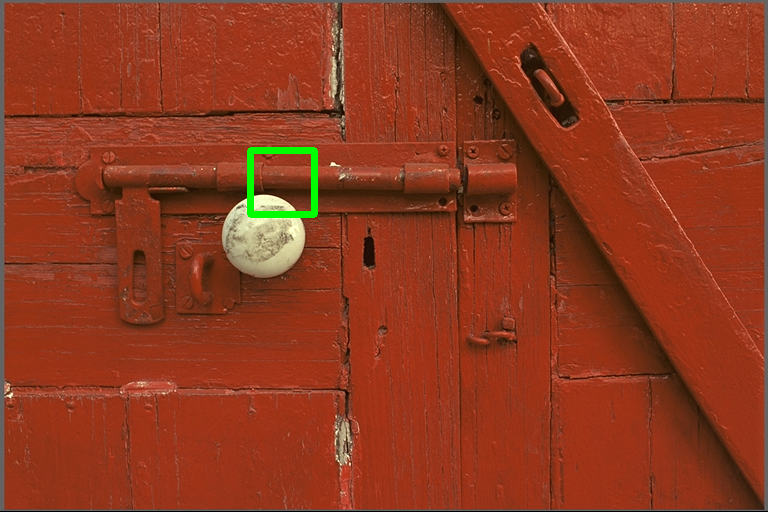
\includegraphics[height=0.14\textwidth]{images/Clean.png}} &
         \fbox{
\includegraphics[height=0.14\textwidth]{images/Noisy_cropped.png}} & 
         \fbox{
\includegraphics[height=0.14\textwidth]{images/CBM3D_cropped.png}} & 
         \fbox{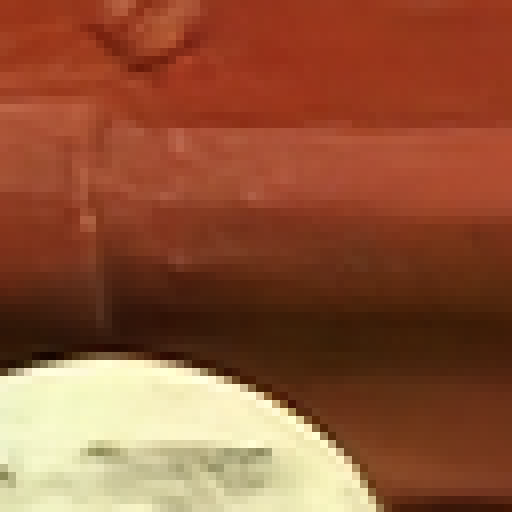
\includegraphics[height=0.14\textwidth]{images/N2C_cropped.png}} &
         \fbox{
\includegraphics[height=0.14\textwidth]{images/SSDN_mu_cropped.png}} &
         \fbox{
\includegraphics[height=0.14\textwidth]{images/SSDN_cropped.png}} \\ 
         \makecell{Test Image\\ (KODAK-2)} & \makecell{Input\\ 20.59 dB} & \makecell{CBM3D\\ 32.44 dB} & \makecell{N2C\\ 32.80 dB} & \makecell{SSDN ($\mu$)\\ 31.38 dB} & \makecell{SSDN\\32.73 dB}
    \end{tabular}
    \caption{Results of applying SSDN and Baselines to Gaussian ($\sigma=25$ noise [$\sigma$ known])}
    \label{fig:images-psnr}
\end{figure}


\section{Discussion}
Despite constraints in breadth of models trained and training durations, a range of results were reproduced from the original paper with relative comparisons against the baselines showing the expected trends. Results in Table \ref{tab:eval_psnrs} correspond to the results shown in Table 1 of the original paper, covering validation performance of: CBM3D, N2C, N2N and different configurations of SSDN. A major claim is that SSDN's training performance matches that of N2C; this was reproducible even when $\sigma$ was not known as can be seen in Figure \ref{fig:training_performance}. Likewise, visual checks using Figure \ref{fig:images-psnr} show very little detail difference between N2C and SSDN. Validation performance with $\sigma$ known also manages to exceed that of CBM3D as expected. In validation, SSDN is expected to achieve an average PSNR of 31.73dB (on BSD300 and KODAK); with a known sigma across the same datasets; the reproduced results show a similar 31.63dB average PSNR, only 0.1dB less with one tenth of the training iterations. Since the number of training iterations in these experiments is lower than that used in the original paper, it is not possible to verify the performance of the fully trained network, however the trend of all plots indicate that further training would keep increasing PSNR for all models. One discrepancy noted between the paper and its results, as well as the reproduced results, is a claim made in the abstract that the methods introduced improve images quality, however they are only ever seen to at best match the state-of-the-art results, rather that exceed them.

One key claim of this paper is that it achieves improved training efficiency compared to state-of-the-art self-supervised denoising methods. The original paper suggests training the N2V baseline by maintaining a smoothed network created from an exponential moving average of previous weights; this is not suggested by \cite{noise2void}. The reproduced baseline results (Figure \ref{fig:training_performance}), which do not do this, indicate that the implementation of SSDN does indeed learn at a higher rate (PSNR achieved in same iterations) than N2V. However, it should be noted that the training time per iteration for SSDN was $4\times$ that of N2V due to loss calculation and the $4\times$ larger network, it is therefore unclear if real-world training performance is improved. 

To verify the implementation, training performance was captured in the same configuration using the original Tensorflow implementation (SSDN-TF in Figure \ref{fig:training_performance}). Although training PSNRs tracked almost exactly, the validation PSNRs from the Tensorflow implementation decreased significantly after approximately 65,000 iterations (this was repeatable for default seed setups). It is not clear why this occurred but may be a quirk in training or highlight a potential issue in their original implementation that was not carried to the PyTorch implementation.

\section{Conclusion}
% Is it a reproducible paper?
When reading the paper, the reader is provided with a detailed account of the theory behind the workings of the paper, as well as justifications for the changes made to the previous solutions to the problem. The provision of the supplement also gave more specific details about the model itself that would not be crucial to the theory, namely details about testing, and the architecture of the network used. The combination of paper and supplement alone was not enough to fully reproduce the results. The authors' code was also required, shedding light on the clipping issue discussed at the end of Section \ref{sec:implementation}. In conclusion, fully utilising a combination of sources allowed for a successful reimplementation and reproduction of results.

\bibliography{references}
\bibliographystyle{iclr2020_conference}

\end{document}
